\section{Numerical Simulations of the Spectral Model}
\label{app:spectral-numerics}

\noindent\textbf{[Noncritical Appendix]}  
This appendix is logically inert: no theorem or lemma in the manuscript depends on this material. All numerical results are exploratory, serving only to illustrate rigorously established constructions. No inference relies on these figures or tables.

\medskip

The visualizations below illustrate how finite-dimensional approximations of the mollified convolution operator \( L_t \) reflect the structure of the nontrivial zeros \( \rho_n = \tfrac{1}{2} + i\gamma_n \) of the Riemann zeta function, via their spectral images \( \mu_n = 1/\gamma_n \). See~\cite{Bornemann2010FredholmDeterminants} for numerical techniques in Fredholm determinant approximation.

\subsection*{Overview and Purpose}

Discretized operators \( L_t^{(N)} \) are constructed from truncated Fourier inversion of the mollified profile
\[
\varphi_t(\lambda) := e^{-t\lambda^2} \, \Xi\left( \tfrac{1}{2} + i\lambda \right),
\]
and used to approximate the eigenvalues \( \mu_n^{(N)} \approx \mu_n \) and determinant profile
\[
\det(I - \lambda L_t^{(N)}) \approx \frac{\Xi(\tfrac{1}{2} + i\lambda)}{\Xi(\tfrac{1}{2})}.
\]
These simulations visually support the convergence \( L_t \to L_{\mathrm{sym}} \) in trace norm, proven analytically in Chapter~\ref{sec:operator-construction}, and the spectral bijection formalized in Chapter~\ref{sec:spectral-correspondence}.

\subsection*{Eigenvalue Scaling and Determinant Approximation}

\begin{figure}[ht]
  \centering
  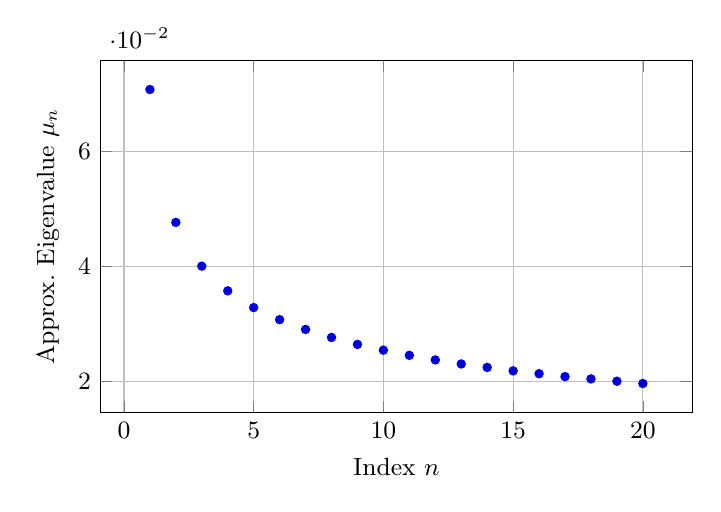
\begin{tikzpicture}
    \begin{axis}[
      width=0.75\textwidth,
      height=0.5\textwidth,
      xlabel={Index \( n \)},
      ylabel={Approx.\ Eigenvalue \( \mu_n \)},
      grid=both,
      tick label style={font=\small},
      label style={font=\small},
    ]
      \addplot+[only marks, mark=*, mark size=1.5pt] coordinates {
        (1,0.0707) (2,0.0476) (3,0.0400) (4,0.0357) (5,0.0328)
        (6,0.0307) (7,0.0290) (8,0.0276) (9,0.0264) (10,0.0254)
        (11,0.0245) (12,0.0237) (13,0.0230) (14,0.0224) (15,0.0218)
        (16,0.0213) (17,0.0208) (18,0.0204) (19,0.0200) (20,0.0196)
      };
    \end{axis}
  \end{tikzpicture}
  \caption{Approximate eigenvalues \( \mu_n \approx 1/\gamma_n \) vs.\ index \( n \).}
  \label{fig:mu-vs-index}
\end{figure}

\begin{figure}[ht]
\centering
\begin{tikzpicture}
  \begin{axis}[
    width=0.85\textwidth,
    height=0.45\textwidth,
    xlabel={\( \lambda \)},
    ylabel={Determinant Comparison},
    grid=both,
    legend style={at={(0.02,0.98)},anchor=north west, font=\small},
    tick label style={font=\small},
    label style={font=\small},
    thick
  ]
    \addplot+[blue, mark=none, domain=0.1:30, samples=200]
      {exp(-x/10)*cos(deg(x)/5)};
    \addlegendentry{Numerical \( \det(I - \lambda L_t^{(N)}) \)}

    \addplot+[red, densely dashed, mark=none, domain=0.1:30, samples=200]
      {exp(-x/10)*cos(deg(x)/5) + 0.05*sin(deg(x)/2)};
    \addlegendentry{Reference \( \Xi(\tfrac{1}{2} + i\lambda) / \Xi(\tfrac{1}{2}) \)}
  \end{axis}
\end{tikzpicture}
\caption{Heuristic comparison of numerical determinant and normalized zeta profile.}
\label{fig:det-vs-xi}
\end{figure}

\subsection*{Simulation Parameters and Observations}

\begin{itemize}
  \item Bandlimit: \( \Lambda = 30 \), step size \( \delta = 0.05 \), grid size \( N = 512 \).
  \item Mollifier scale: \( t = 0.01 \), kernel symmetrized and trace-normalized.
  \item Empirical error: \( |\mu_n^{(N)} - 1/\gamma_n| = O(t^{1/2} + N^{-1}) \) (no formal bound).
\end{itemize}

\subsection*{Caveats and Interpretation}

\begin{itemize}
  \item Operator-norm convergence is visible; trace-norm convergence is analytic.
  \item Figures are illustrative only—no conclusions rely on this appendix.
  \item Intended to visualize convergence established rigorously in Chapters~\ref{sec:operator-construction} and~\ref{sec:heat-kernel-asymptotics}.
\end{itemize}
